\chapter{OLS 估计的无偏性}
\label{ch:week4}
\section{简单 OLS：概念、假设与定理}
\sourcepage{4}{1}{4/1}
\label{sec:unbiasedness-concept}
学习目标：
\begin{enumerate}
\item 陈述保证\hy{有限样本无偏性}的假设。
\item 用经济语言解释零条件均值。
\item 判断常见情形下遗漏变量偏误的方向。
\end{enumerate}
\subsection{估计与拟合优度回顾}
\[y=\beta_0+\beta_1x+u,\qquad
\hat y=\hat\beta_0+\hat\beta_1x,\]
\[\hat\beta_1=\frac{\Cov_n(x,y)}{\Var_n(x)},\qquad
\hat\beta_0=\bar y-\hat\beta_1\bar x,\qquad
R^2=\frac{\ESS}{\TSS}=1-\frac{\RSS}{\TSS}.\]
此处的 $R^2$ 恒等式要求模型含截距，且 TSS 为正。

\subsection{总体参数与估计量}
\begin{description}
\item[$\beta_j$。]固定但未知的总体参数。
\item[$\hat\beta_j$。]由随机样本计算的估计量。在观测样本之前，它是随机变量，会随样本改变，具有抽样分布；相应的矩在存在时才有定义。
\end{description}
在某个具体样本中，估计值可能高于或低于 $\beta_j$；并不要求它等于真值，也不能一般地预期每次都会相等。\corr{estimator-estimate}

\begin{definition}[无偏估计量]
若 $\theta$ 的估计量 $\hat\theta$ 的期望存在，并且
\[\hm{\E[\hat\theta]=\theta}.\]
则称该估计量\hy{无偏}。对于 OLS，我们寻找使 $\E[\hat\beta_0]=\beta_0$ 与 $\E[\hat\beta_1]=\beta_1$ 成立的条件。
\end{definition}
在重复抽样中，估计量的期望等于真实总体参数。在任意一个样本中，估计值仍可能明显偏离真值。\blue{无偏性描述重复抽样的平均表现，不保证某一次估计恰好正确，也不保证估计误差很小。}

\subsection{假设概览}
\begin{enumerate}[label=SLR\arabic*.]
\item 对参数线性：$y=\beta_0+\beta_1x+u$。
\item 随机抽样：$\{(x_i,y_i):i=1,\ldots,n\}$ 是来自总体模型的独立同分布观测。
\item 样本存在变异：$S_{xx}=\sum_i(x_i-\bar x)^2>0$。
\item 零条件均值：$\E[u\mid x]=0$。
\end{enumerate}
\added{若要陈述无条件无偏性，还须假设 OLS 估计量几乎处处有定义，且下文使用的期望存在。这里的均值无偏结论不要求误差正态分布，也不要求同方差。}

\subsection{简单 OLS 假设的详细说明}
\sourcepage{4}{2}{4/2}
\paragraph{SLR1：对参数线性。}
\[\hy{$y=\beta_0+\beta_1x+u$}.\]
未知系数以线性形式进入模型。可以对已观测变量作变换，而不必使模型对参数变为非线性。

\paragraph{SLR2：随机抽样。}
每个观测满足 $y_i=\beta_0+\beta_1x_i+u_i$。观测对 $(x_i,y_i)$ 在不同 $i$ 之间相互独立且同分布。因此，对 $i\ne j$，$u_i=y_i-\beta_0-\beta_1x_i$ 与 $u_j$ 独立；但这并不表示 $u_i$ 与其自身的回归变量 $x_i$ 独立。
\begin{figure}[htbp]
\centering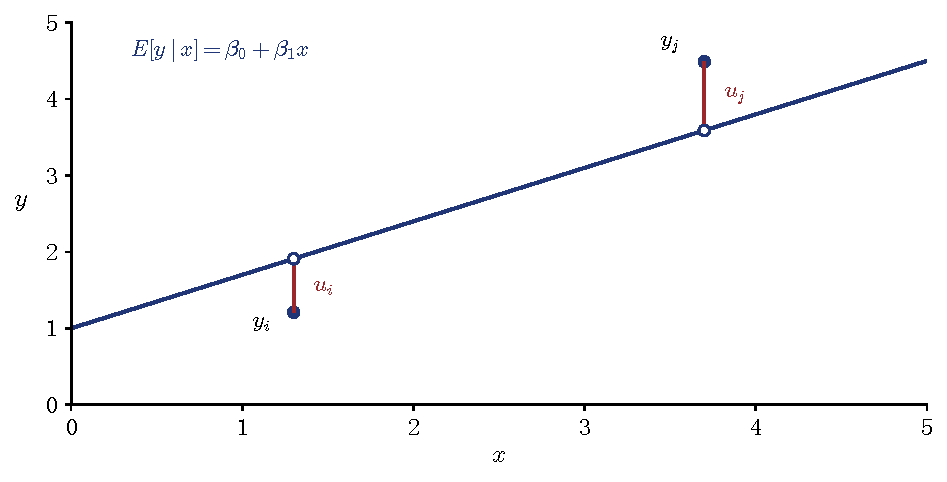
\includegraphics[width=.79\linewidth]{population_errors.pdf}
\caption{总体误差是观测值偏离条件均值的垂直距离，不是相对于估计回归线的残差。本图沿用原稿中的两个观测点示意，点的位置不代表真实数据。}
\label{fig:population-errors}
\end{figure}

\paragraph{SLR3：回归变量存在变异。}
观测到的 $x_i$ 不能全部取相同值：
\[\hy{$S_{xx}=\sum_i(x_i-\bar x)^2>0$}.\]
若所有 $x_i$ 都相同，斜率公式的分母为零，无法分别确定截距和斜率。

\paragraph{SLR4：零条件均值。}
\[\hy{$\E[u_i\mid x_i]=0$}\qquad(i=1,\ldots,n).\]
解释变量取任何值时，未观测因素的条件平均值均为零。在独立抽样下，这还意味着
\[\E[u_i\mid\mathcal X]=0,\qquad\mathcal X=(x_1,\ldots,x_n),\]
因为给定 $x_i$ 后，其他观测的回归变量不再提供有关 $u_i$ 的额外信息。证明中须以\emph{整个已观测样本设计}为条件，因为抽样前 $S_{xx}$ 是随机的。\corr{conditioning}

\begin{theorem}[简单 OLS 的无偏性]\label{thm:simple-unbiased}
在 SLR1--SLR4 及前述存在性条件成立时，
\[\E[\hat\beta_0\mid\mathcal X]=\beta_0,\qquad
\E[\hat\beta_1\mid\mathcal X]=\beta_1.\]
因此，$\E[\hat\beta_0]=\beta_0$，且 $\E[\hat\beta_1]=\beta_1$。
\end{theorem}

\subsection{斜率的无偏性证明}
逐步展开斜率公式：
\begin{align}
\hat\beta_1
&=\frac{\sum_i(x_i-\bar x)(y_i-\bar y)}{S_{xx}}
=\frac{\sum_i(x_i-\bar x)y_i}{S_{xx}}\notag\\
&=\frac{\sum_i(x_i-\bar x)(\beta_0+\beta_1x_i+u_i)}{S_{xx}}\notag\\
&=\frac{\beta_0\sum_i(x_i-\bar x)
+\beta_1\sum_i(x_i-\bar x)x_i+\sum_i(x_i-\bar x)u_i}{S_{xx}}.\label{eq:slope-expansion}
\end{align}
注意 $\sum_i(x_i-\bar x)=0$，并且
\begin{align*}
S_{xx}&=\sum_i(x_i^2-2x_i\bar x+\bar x^2)
=\sum_i x_i^2-n\bar x^2\\
&=\sum_i x_i(x_i-\bar x).
\end{align*}
因此，
\begin{equation}\label{eq:slope-error}
\hm{\hat\beta_1=\beta_1+\frac{\sum_i(x_i-\bar x)u_i}{S_{xx}}}.
\end{equation}
\begin{align*}
\E[\hat\beta_1\mid\mathcal X]
&=\beta_1+\frac{\sum_i(x_i-\bar x)\E[u_i\mid\mathcal X]}{S_{xx}}\\
&=\beta_1.
\end{align*}
最后，$\E[\hat\beta_1]=\E\{\E[\hat\beta_1\mid\mathcal X]\}=\beta_1$。\red{不能在无条件期望中直接把随机分母 $S_{xx}$ 提到期望外。}\corr{conditioning}

\subsection{截距的无偏性证明：考试提示}
\sourcepage{4}{3}{4/3}
\label{sec:intercept-proof}
对模型取样本平均，有
\[\bar y=\beta_0+\beta_1\bar x+\bar u,\qquad
\bar u=\frac1n\sum_i u_i.\]
将其代入 $\hat\beta_0=\bar y-\hat\beta_1\bar x$：
\[\hat\beta_0=\beta_0+(\beta_1-\hat\beta_1)\bar x+\bar u.\]
于是，
\begin{align*}
\E[\hat\beta_0\mid\mathcal X]
&=\beta_0+\bar x\bigl(\beta_1-\E[\hat\beta_1\mid\mathcal X]\bigr)
+\E[\bar u\mid\mathcal X]\\
&=\beta_0+\bar x(\beta_1-\beta_1)+0=\beta_0.
\end{align*}
$\bar u$ 项前应为\emph{加号}；手写证明中间一行出现了不一致的减号，此处已更正。\corr{intercept-sign}
再由迭代期望法则，得 $\E[\hat\beta_0]=\beta_0$。

\subsection{讨论：假设不成立会怎样？}
\blue{原稿在此处另有课堂时间标记：15 分钟。}
\begin{description}
\item[SLR1：对参数线性。]若模型对未知系数非线性，就超出了这里的线性 OLS 证明范围。\blue{非线性参数与变量的非线性变换要区分。}
\item[SLR2：随机抽样。]原稿列举了时间序列中的序列相关（自相关）、不具代表性的样本和观测间的溢出效应。这些情况可能违背所述独立同分布设定，或引发样本代表性与模型设定问题。但它们本身\emph{不能}证明每个 OLS 系数都有偏；还必须另行检查条件均值限制。\corr{violations}
\item[SLR3：样本变异。]若 $S_{xx}=0$，简单回归的斜率便无法与截距分别识别。
\item[SLR4：零条件均值。]在观测性研究中，遗漏因素可能与回归变量相关。若 $\Cov(x,u)\ne0$，ZCM 不可能成立。但 ZCM 比零协方差更强：$\Cov(x,u)=0$ 不能推出 $\E[u\mid x]=0$。单凭 ZCM 失败，也不能保证每种设计下都必然存在非零的有限样本偏差。\corr{zcm-covariance}
\end{description}
\added{原稿中的协方差恒等式为
\[\Cov(x,u)=\E[xu]-\E[x]\E[u].\]
在相应矩存在时，ZCM 同时推出 $\E[u]=0$ 与 $\E[xu]=0$。反方向一般不成立。}

\section{多元 OLS：假设与定理}
\sourcepage{4}{4}{4/5}
\label{sec:multiple-unbiased}
\subsection{MLR1：对参数线性}
总体模型为
\[y=\beta_0+\beta_1x_1+\beta_2x_2+\cdots+\beta_kx_k+u.\]
系数 $\beta_0,\ldots,\beta_k$ 是所关心的未知常数；$u$ 为误差项。

\subsection{MLR2：随机抽样}
从该总体模型取得 $n$ 个独立同分布的观测向量
\[\{(x_{1i},\ldots,x_{ki},y_i):i=1,\ldots,n\}\]
因此，$y_i=\beta_0+\sum_{j=1}^k\beta_jx_{ji}+u_i$。

\subsection{MLR3：不存在完全共线性}
包含截距列的样本设计矩阵具有满列秩。除截距外，任何回归变量都不是常数，也不存在某一列是其他列的精确线性组合。\blue{相关可以存在；完全线性的重复信息会使单独系数无法识别。}

\begin{example}[完全共线性]
保留原稿中的所有例子：
\begin{enumerate}
\item 常数回归变量：模型已含截距，却又加入 $x_1=10$。
\item 精确倍数或仿射关系：$x_1=2x_2$，或 $x_1=a+bx_2$。
\item 精确线性组合：$x_3=x_1+x_2$。
\end{enumerate}
\begin{figure}[htbp]
\centering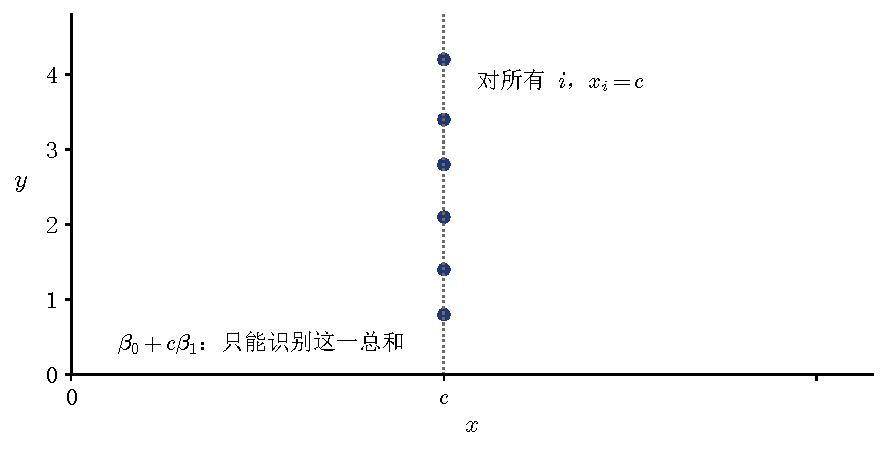
\includegraphics[width=.72\linewidth]{no_sample_variation.pdf}
\caption{若每个观测均有 $x_i=c$，只能识别 $\beta_0+c\beta_1$。本图以示意点重现原稿中 $x$ 为常数的情形。}
\label{fig:no-variation}
\end{figure}
若回归已包含 $\ln(\mathrm{income})$，再加入 $2\ln(\mathrm{income})$ 会造成完全共线性。同样，若总支出 $=$ 支出 A $+$ 支出 B，则同时纳入这三个变量也会造成完全共线性。

仅保留支出 A 与 B、删去它们的精确总和，并不会因此产生上述特定的共线关系。以下模型
\[y=\beta_0+\beta_1\ln(\mathrm{income})
+\beta_2[\ln(\mathrm{income})]^2+u\]
并\emph{不自动}具有完全共线性：变量的平方一般不是其水平值的仿射变换。\blue{它对变量可以非线性，但对参数仍线性。}不过，在取值种类过少等特殊样本中，设计矩阵仍可能不满秩。\corr{collinearity}
\end{example}


\subsection{MLR4：零条件均值}
\sourcepage{4}{5}{4/6}
\[\hm{\E[u\mid x_1,x_2,\ldots,x_k]=0}.\]
解释变量不能系统地预测误差的条件均值。在本笔记的术语中，这称为均值外生性条件。\red{它推出与误差不相关；仅仅不相关不足以推出这个条件。}\corr{zcm-covariance}
原稿区分了外生回归变量与内生回归变量。在结构模型中，若回归变量与 $u$ 中遗漏的决定因素相关，就可能存在内生性；与\emph{拟合残差}的样本协方差为零，不能排除这一问题。

\begin{theorem}[多元 OLS 的无偏性]\label{thm:multiple-unbiased}
在 MLR1--MLR4 成立、样本设计矩阵几乎处处满秩且相关期望存在时，
\[\E[\hat\beta_j\mid\mathcal X]=\beta_j,
\qquad\E[\hat\beta_j]=\beta_j,\qquad j=0,1,\ldots,k,\]
其中，$\mathcal X$ 表示整个已观测回归变量矩阵。
\end{theorem}

\subsection{利用剔除线性影响进行证明}
\label{sec:fwl-week4}
固定一个回归变量 $x_j$。按原稿的方法，将它对常数项及全部其他回归变量回归：
\begin{equation}\label{eq:auxiliary-j}
x_{ji}=\hat\delta_0+\sum_{\ell\ne j}\hat\delta_\ell x_{\ell i}+\hat r_{ji}.
\end{equation}
\blue{不同样本会有不同的辅助回归系数和残差。给定整组 $\mathcal X$，这些量都是已确定的。}
辅助回归的正规方程给出
\[\sum_i\hat r_{ji}=0,\qquad
\sum_i x_{\ell i}\hat r_{ji}=0\quad(\ell\ne j).\]
定义\emph{辅助回归}的残差平方和
\[S_{r_jr_j}=\sum_i\hat r_{ji}^{\,2}>0.
\]
这就是原稿记作“$\RSS_j$”的量，应与因变量回归的残差平方和区分。由于 $x_{ji}$ 等于其辅助回归拟合部分加上 $\hat r_{ji}$，有
\[\sum_i\hat r_{ji}x_{ji}=\sum_i\hat r_{ji}^{\,2}=S_{r_jr_j}.
\]
FWL 的单侧系数形式给出
\begin{align}
\hat\beta_j
&=\frac{\Cov_n(\hat r_j,y)}{\Var_n(\hat r_j)}
=\frac{\sum_i\hat r_{ji}y_i}{S_{r_jr_j}}\notag\\
&=\frac{\sum_i\hat r_{ji}\left(\beta_0+\sum_{\ell=1}^k\beta_\ell x_{\ell i}+u_i\right)}{S_{r_jr_j}}\notag\\
&=\hm{\beta_j+\frac{\sum_i\hat r_{ji}u_i}{S_{r_jr_j}}}.\label{eq:multiple-slope-error}
\end{align}
其余回归变量项都因辅助回归的正交性而消失。取条件期望，得
\[\E[\hat\beta_j\mid\mathcal X]
=\beta_j+\frac{\sum_i\hat r_{ji}\E[u_i\mid\mathcal X]}{S_{r_jr_j}}
=\beta_j.\]
由迭代期望法则，即可证明每个斜率的无条件无偏性。
\added{截距可由下式处理：
\[\hat\beta_0=\bar y-\sum_{j=1}^k\hat\beta_j\bar x_j
=\beta_0+\bar u+\sum_{j=1}^k(\beta_j-\hat\beta_j)\bar x_j.\]
给定 $\mathcal X$ 后，每个 $\bar x_j$ 都是固定的；利用斜率的结论及 $\E[\bar u\mid\mathcal X]=0$，得到 $\E[\hat\beta_0\mid\mathcal X]=\beta_0$。}

\section{假设汇总与无偏性}
\sourcepage{4}{6}{4/7}
\label{sec:assumptions-summary}
\paragraph{核心：控制其他因素。}
多元回归的核心能力是通过 FWL 排除其他已观测因素的线性影响，识别某一自变量剩余变化与结果的关系。\blue{“纯净影响”的因果说法仍依赖适当的模型与外生性，不能仅由控制操作保证。}

\paragraph{无偏性的本质：重复抽样的平均性质.}
单次抽样的具体估计是一个已经实现的数值；生成这些数值的 OLS 估计程序才有统计意义上的无偏性。

\subsection{四项假设的并列比较}
\begin{center}
\small\renewcommand{\arraystretch}{1.35}
\begin{tabular}{P{3.1cm}P{5.35cm}P{6.3cm}}
\toprule
假设 & 简单回归 & 多元回归\\
\midrule
对参数线性 & $y=\beta_0+\beta_1x+u$ & $y=\beta_0+\sum_{j=1}^k\beta_jx_j+u$\\
随机抽样 & 独立同分布的观测对 $(x_i,y_i)$ & 独立同分布的观测向量 $(x_{1i},\ldots,x_{ki},y_i)$\\
样本秩 & $\sum_i(x_i-\bar x)^2>0$ & 含常数列在内的设计矩阵各列之间，不存在精确线性关系\\
零条件均值 & $\E[u\mid x]=0$ & $\E[u\mid x_1,\ldots,x_k]=0$\\
\bottomrule
\end{tabular}
\end{center}

\begin{example}[某次教育回报率估计]\label{ex:unbiased-number}
原稿给出
\[\widehat{\ln(\wage)}
=0.284+0.092\educ+0.0041\,\mathrm{exper}+0.022\,\mathrm{tenure}.\]
若 MLR1--MLR4 成立，能否说“$9.2\%$ 是教育回报率的无偏估计”？

\red{无偏性属于估计量的性质。}数值 $0.092$ 是某一次估计的实现值。准确表述是：在所述假设下，对数工资方程中教育系数的 OLS 估计量无偏；它在本样本中的实现值为 $0.092$。

原稿中的“$9.2\%$”是教育年限增加一年时的近似百分比解释。保持误差不变时，精确的百分比变换为
\[100(e^{0.092}-1)\simeq9.64\%.
\]
\added{即使 $\hat\beta$ 是 $\beta$ 的无偏估计量，非线性变换 $e^{\hat\beta}-1$ 也未必是 $e^\beta-1$ 的无偏估计量。此外，拟合对数工资本身并不能识别教育的因果回报，也不能直接给出工资水平值的条件均值。}\corr{unbiased-log}
\end{example}

\section{模型设定与偏误}
\sourcepage{4}{7}{4/8}
\label{sec:model-specification}
这里区分两种模型设定：\hy{过度设定}，即加入无关变量；\hy{不足设定}，即遗漏相关变量。

\subsection{加入无关变量}
从以下模型出发：
\[y=\beta_0+\beta_1x_1+\beta_2x_2+u.\]
现在估计一个额外包含 $x_3$ 的模型，其总体系数 $\beta_3=0$。扩充后的样本设计仍须满秩，即 $x_3$ 不能是已有设计矩阵各列的精确线性组合。

若\emph{扩充后}的外生性条件成立，
\[\E[u\mid x_1,x_2,x_3]=0,
\]
则完整模型中的 OLS 估计量仍无偏：
\[\E[\hat\beta_j]=\beta_j\quad(j=0,1,2),\qquad
\E[\hat\beta_3]=0.
\]
\red{但仅有 $\E[u\mid x_1,x_2]=0$，并不能推出 $\E[u\mid x_1,x_2,x_3]=0$。}加入一个与误差相关的回归变量，会改变条件均值限制。某个系数为零，本身不能证明该新增控制变量具有外生性。\corr{irrelevant-exogeneity}

\added{在同方差、固定设计模型下，若加入无关变量减少了原有某个回归变量的残差变异，则该变量斜率的真实条件方差弱增，即不会下降。这不保证严格增加，也不保证某一次计算出的估计标准误一定上升。原稿中的“方差增加”须附带这些限定。}\corr{irrelevant-variance}

\subsection{遗漏相关变量}
\label{sec:ovb-sample}
设真实的长模型为
\[y_i=\beta_0+\beta_1x_i+\beta_2z_i+u_i,\qquad
\E[u_i\mid x_i,z_i]=0.\]
其拟合形式为
\[y_i=\hat\beta_0+\hat\beta_1x_i+\hat\beta_2z_i+\hat u_i.
\]
若 $z$ 未被观测或被遗漏，短回归将 $y$ 对 $(1,x)$ 回归：
\[y_i=\hat{\tilde\beta}_0+\hat{\tilde\beta}_1x_i+\hat v_i,
\qquad v_i=\beta_2z_i+u_i\ \text{（结构方程中的误差）}.
\]
当遗漏部分与 $x$ 相关时，遗漏一个相关变量才会影响 $x$ 的斜率；仅仅“该变量影响因变量”还不够。\corr{omitting-relevant}

\paragraph{短回归与长回归的精确样本恒等式。}
精确的样本关系为
\begin{equation}\label{eq:sample-ovb}
\hm{\hat{\tilde\beta}_1=\hat\beta_1+\hat\beta_2\hat\delta_1},
\end{equation}
其中，$\hat\delta_1$ 来自辅助 OLS 回归
\[z_i=\hat\delta_0+\hat\delta_1x_i+\hat r_i,
\qquad
\hat\delta_1=\frac{\sum_i(x_i-\bar x)(z_i-\bar z)}{S_{xx}}.
\]
首先，长模型残差与 $x$ 及常数项在样本中正交：
\begin{align*}
\sum_i(x_i-\bar x)(\hat u_i-\bar{\hat u})
&=\sum_i x_i\hat u_i-\bar x\sum_i\hat u_i\\
&=0.
\end{align*}
将去均值后的长模型拟合方程代入短回归斜率公式，得
\begin{align*}
\hat{\tilde\beta}_1
&=\frac{\sum_i(x_i-\bar x)(y_i-\bar y)}{S_{xx}}\\
&=\frac{\sum_i(x_i-\bar x)\left[\hat\beta_1(x_i-\bar x)
+\hat\beta_2(z_i-\bar z)+(\hat u_i-\bar{\hat u})\right]}{S_{xx}}\\
&=\hat\beta_1+\hat\beta_2\frac{\sum_i(x_i-\bar x)(z_i-\bar z)}{S_{xx}}+0\\
&=\hat\beta_1+\hat\beta_2\hat\delta_1.
\end{align*}
这是同一个具体样本中的代数恒等式，此处尚未取期望。

\subsection{期望偏差：哪些量是随机的？}
\sourcepage{4}{8}{4/9}
\label{sec:ovb-expectation}
现在令 $\mathcal X$ 包含样本中的全部 $x_i$ 与 $z_i$。在有效的长模型下，
\[\E[\hat\beta_1\mid\mathcal X]=\beta_1,
\qquad\E[\hat\beta_2\mid\mathcal X]=\beta_2.
\]
\emph{给定}这一设计后，辅助斜率 $\hat\delta_1$ 是固定的。因此，
\begin{align}
\E[\hat{\tilde\beta}_1\mid\mathcal X]
&=\E[\hat\beta_1+\hat\beta_2\hat\delta_1\mid\mathcal X]\notag\\
&=\hm{\beta_1+\beta_2\hat\delta_1},\label{eq:ovb-conditional}\\
\E[\hat{\tilde\beta}_1]
&=\beta_1+\beta_2\E[\hat\delta_1].\label{eq:ovb-unconditional}
\end{align}
等价地，保留原稿利用迭代期望的推导路线：
\begin{align*}
\E[\hat\beta_2\hat\delta_1]
&=\E\{\E[\hat\beta_2\hat\delta_1\mid\mathcal X]\}\\
&=\E\{\hat\delta_1\E[\hat\beta_2\mid\mathcal X]\}
=\beta_2\E[\hat\delta_1].
\end{align*}
\added{若要得到原稿中的有限样本表达式
\[\E[\hat{\tilde\beta}_1]=\beta_1+\beta_2\delta_1,\]
还需要 $\E[\hat\delta_1]=\delta_1$。一个充分的附加条件是辅助条件均值设定正确：
\[\E[z\mid x]=\delta_0+\delta_1x\]
并满足随机抽样、样本变异及所需可积性条件。仅将 $\delta_1$ 定义为总体投影斜率，并不能自动建立上述有限样本等式。}\corr{ovb-levels}

对于\emph{总体线性投影}，即使不增加上述线性条件均值假设，斜率差仍为
\[\tilde\beta_1-\beta_1=\beta_2\delta_1,
\qquad\delta_1=\frac{\Cov(x,z)}{\Var(x)}.
\]
在通常的一致性条件下，它也描述渐近的斜率差。总体与渐近结论不应和精确样本恒等式或有限样本期望混淆。

\subsection{遗漏变量偏误的方向}
若适用的斜率差或偏差为 $B=\beta_2\delta_1$，则
\begin{description}
\item[上偏。]$B>0$：短回归斜率高于目标 $\beta_1$。
\item[下偏。]$B<0$：短回归斜率低于目标 $\beta_1$。
\item[无偏差。]$B=0$，例如 $\beta_2=0$ 或 $\delta_1=0$。
\end{description}
当 $\Var(x)>0$ 时，$\delta_1$ 与 $\Cov(x,z)$ 同号。原稿的符号表写为
\begin{center}
\renewcommand{\arraystretch}{1.4}
\begin{tabular}{lcc}
\toprule
 & $\Cov(x,z)>0$ ($\delta_1>0$) & $\Cov(x,z)<0$ ($\delta_1<0$)\\
\midrule
$\beta_2>0$ & \hy{上偏} & 下偏\\
$\beta_2<0$ & 下偏 & \hy{上偏}\\
\bottomrule
\end{tabular}
\end{center}
\blue{该表直接适用于总体投影差；用于有限样本平均偏差时，应满足上一小节的附加条件。给定样本设计的偏差方向则由 $\hat\delta_1$ 决定。}

\paragraph{向零偏。}
当 $\beta_1$ 为正时，向零移动意味着下偏；当 $\beta_1$ 为负时，向零移动意味着上偏。若采用通常的衰减解释，偏移后的系数必须仍位于目标值与零之间。\red{方向正确但越过零，不能仅凭上偏或下偏就称为向零偏。}\corr{toward-zero}

\subsection*{本章小结}
\addcontentsline{toc}{subsection}{本章小结}
\begin{itemize}
\item 无偏性是估计量在重复抽样下的期望性质。
\item 样本设计满秩和零条件均值支撑了条件期望证明；仅有零协方差是更弱的条件。
\item 加入有效的无关控制变量可保持无偏性，但可能降低精度。遗漏既影响结果又与保留变量相关的回归变量，会改变斜率。
\item 应区分样本恒等式、条件偏差、无条件有限样本偏差与总体投影差。
\end{itemize}
